\newcommand{\nom}{Production Éolienne/Solaire}
\newcommand{\sequence}{1}
\newcommand{\numero}{02}
\newcommand{\type}{DS}
\newcommand{\descrip}{Production Éolienne/Solaire}

\documentclass[10pt,a4paper]{article}
  \usepackage[french]{babel}
  \usepackage[utf8]{inputenc}
  \usepackage[T1]{fontenc}
  \usepackage{xcolor}
  \usepackage[]{graphicx}
  \usepackage{makeidx}
  \usepackage{textcomp}
  \usepackage{amsmath}
  \usepackage{amssymb}
  \usepackage{stmaryrd}
  \usepackage{fancyhdr}
  \usepackage{lettrine}
  \usepackage{calc}
  \usepackage{boxedminipage}
  \usepackage[french,onelanguage, boxruled,linesnumbered]{algorithm2e}
  \usepackage[colorlinks=false,pdftex]{hyperref}
  \usepackage{minted}
  \usepackage{url}
  %\usepackage[locale=FR]{siunitx}
  \usepackage{multicol}
  \makeindex

  %\graphicspath{{../Images/}}

%  \renewcommand\listingscaption{Programme}

  %\renewcommand{\thechapter}{\Alph{chapter}}
  \renewcommand{\thesection}{\Roman{section}}
  %\newcommand{\inter}{\vspace{0.5cm}%
  %\noindent }
  %\newcommand{\unite}{\ \textrm}
  \newcommand{\ud}{\mathrm{d}}
  \newcommand{\vect}{\overrightarrow}
  %\newcommand{\ch}{\mathrm{ch}} % cosinus hyperbolique
  %\newcommand{\sh}{\mathrm{sh}} % sinus hyperbolique

  \textwidth 160mm
  \textheight 250mm
  \hoffset=-1.70cm
  \voffset=-1.5cm
  \parindent=0cm

  \pagestyle{fancy}
  \fancyhead[L]{\bfseries {\large PTSI -- Dorian}}
  \fancyhead[C]{\bfseries{{\type} {\num}}}
  \fancyhead[R]{\bfseries{\large Informatique}}
  \fancyfoot[C]{\thepage}
  \fancyfoot[L]{\footnotesize R. Costadoat, J. Genzmer, W. Robert}
  \fancyfoot[R]{\small \today}
  
  \definecolor{bg}{rgb}{0.9,0.9,0.9}
  
  
  % macro Juliette
  
\usepackage{comment}   
\usepackage{amsthm}  
\theoremstyle{definition}
\newtheorem{exercice}{Exercice}
\newtheorem*{rappel}{Rappel}
\newtheorem*{remark}{Remarque}
\newtheorem*{defn}{Définition}
\newtheorem*{ppe}{Propriété}
\newtheorem{solution}{Solution}

%%\usepackage[a4paper]{geometry}
%\geometry{margin={1cm,1.2cm}}
%\usepackage[francais]{babel}
%\usepackage{nopageno} %pas de numérotation de page
%\pagestyle{plain} %numérotation en bas de page, pas d'entête
%\usepackage{hyperref}
%\usepackage[latin1]{inputenc}

%%%%%%%%%%%%%%%%%%%%%%%%%%%%%%%%%%%%%%%%%%%%%%%%%%%%%%%%%%%%%%%%%%%%%%%%%%%%%%%%%%%%%

\usepackage{amsthm}
\usepackage{amscd}
%\usepackage{mathrsfs}
%\usepackage{amsfonts}
%\usepackage[T1]{fontenc}
%\usepackage{theorem}
\usepackage{lscape}
\usepackage{variations}  % pour faire des tableaux de variations
\usepackage{dsfont}
\usepackage{fancyvrb} % pour mettre Verbatim dans une box

% Pour les figures
\usepackage{subfig}
%\usepackage{calc} % Pour pouvoir donner des formules dans les d�finitions de longueur
%\usepackage{graphicx} % Pour inclure des graphiques 
% Attention : pour inclure des .jpg comme dans l'exemple (ou des .png ou .pdf)
% il faut compiler directement en pdf (commande pdflatex).
% Pour inclure des .eps, il faut compiler avec latex + dvips + ps2pdf.
\usepackage{psfrag}
%\usepackage{color}

%%%%%%%%%%%%%%%%%%%%%%%%%%%%%%%%%%%%%%%%%%%%%%%%%%%%%%%%%%%%%%%%%%%%%%%%%%%%%%%%%%%%%

\theoremstyle{definition}
\newtheorem*{thm}{Théorème}
%\theorembodyfont{\rmfamily}
\newtheorem*{defn}{Définition}
\newtheorem{exercice}{Exercice}
\newtheorem*{problem}{Problème}
\newtheorem*{prop}{Proposition}
\newtheorem*{corollaire}{Corollaire}
\newtheorem*{lemme}{Lemme}
\newtheorem*{remark}{Remarque}
\newtheorem*{notation}{Notation}
\newtheorem*{ex}{Exemple}
\newtheorem*{ppe}{Propriété}
\newtheorem*{meth}{Méthode}
\newtheorem*{rappel}{Rappel}
\newtheorem*{voca}{Vocabulaire}
\setlength{\columnseprule}{0.5pt}


%%%%%%%%%%%%%%%%%%%%%%%%%%%%%%%%%%%%%%%%%%%%%%%%%%%%%%%%%%%%%%%%%%%%%%%%%%%%%%%%%%%%%

\newcommand{\bi}{\bigskip}
\newcommand{\dsp}{\displaystyle}
\newcommand{\noi}{\noindent}
\newcommand{\ov}{\overline}
\newcommand{\dsum}{\displaystyle \sum}
\newcommand{\dprod}{\displaystyle \prod}
\newcommand{\dint}{\displaystyle \int}
\newcommand{\dlim}{\displaystyle \lim}

%%%%%%%%%%%%%%%%%%%%%%%%%%%%%%%%%%%%%%%%%%%%%%%%%%%%%%%%%%%%%%%%%%%%%%%%%%%%%%%%%%%%%


%\newcommand{\pgcd}{\mathrm{pgcd}} % pgcd
%\providecommand{\norm}[1]{\lVert#1\rVert} % norme
%\DeclareMathOperator{\Tan}{Tan}  % espace tangent


\newcommand{\N}{\mathbb{N}}
\newcommand{\Z}{\mathbb{Z}}
\newcommand{\Q}{\mathbb{Q}}
\newcommand{\R}{\mathbb{R}}
\newcommand{\C}{\mathbb{C}}
\newcommand{\K}{\mathbb{K}}
\newcommand{\U}{\mathbb{U}}
\newcommand{\Tr}{\text{Tr}\,}
\newcommand{\pg}{\geqslant}
\newcommand{\pp}{\leqslant}
\newcommand{\bul}{\item[$\bullet$]}
\newcommand{\card}{\text{Card}}
\newcommand{\re}{\text{Re}\;}
\newcommand{\im}{\text{Im}\;}
\newcommand{\Ker}{\text{Ker}\;}
\newcommand{\Vect}{\text{Vect}\;}
\newcommand{\rg}{\text{rg}\;}
\newcommand{\TT}{{}^t\!}
%\newcommand{\sh}{\text{sh}}
%\newcommand{\ch}{\text{ch}}
\newcommand{\Mat}{\text{Mat}}
\usepackage{textcomp}



%%%%%%%%%%%%%%%%%%%%%%%%%%%%%%%%%%%%%%%%%%%%%%%%%%%%%%%%%%%%%%%%%%%%%%%%%%%%%%%%%%%%%%%%%%%%%%%%%%%%%%%%%%%%%%%%%%%%%%%%%%%




\begin{document}

\begin{center}
{\Large\bf TP \no {\numero} -- \descrip}
\end{center}

\section{Import de données}

Jusqu'à présent, lorsque vous avez traité des données avec un programme écrit en python, elles ont disparu à la fermeture du programme car elles étaient stockées dans la mémoire vive de l'ordinateur (Random Access Memory). Pour conserver des données pour une utilisation ultérieure, il faut les stocker sur des mémoires non volatiles (disque dur, carte mémoire, CD Rom,\dots). Elles sont stockées sur ces supports dans une zone physique identifiée par le système d'exploitation\footnote{En anglais « \textit{OS} » (pour \textit{Operating system}.)}. La suite de donnée structurée est appelée fichier (ou \textit{file} en anglais).

Il existe deux types de fichier de données : les fichiers de type texte (encore appelé ASCII) et de type binaire.

Les fichiers de type texte sont constitués de caractères codés par un nombre entier, écrit en code binaire sur 8 bits (1 octet), compris entre 0 et 255.

Les 128 premiers caractères sont communs aux différents codes ASCII. 

Les 128 caractères suivant permettre de décrire les différents caractères nationaux (exemple : é, è, à,\dots pour le français). Chaque code ASCII fait l'objet d'une norme ISO. Pour les langues d'Europe de l'ouest, la norme est ISO 8859-1 appelé Latin-1. Le codage est donné dans le tableau~\ref{fig:tableASCII}.

\begin{figure}[htp]
 \centering
 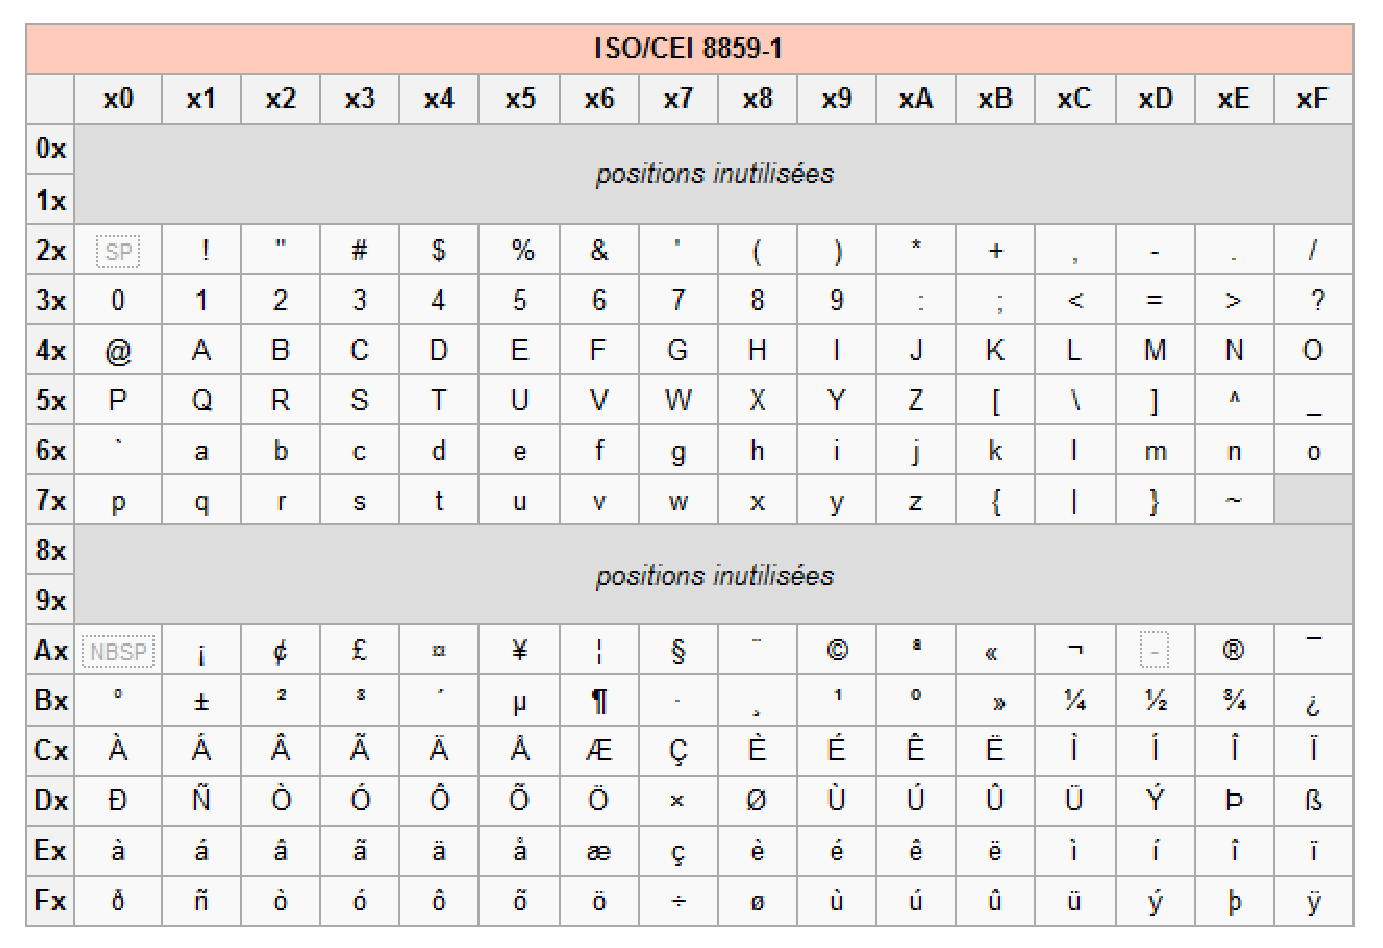
\includegraphics[width=8cm]{img/tableASCII}
 \label{fig:tableASCII}
\end{figure}

L'encodage universel des caractères est réalisé soit par l'Unicode ou l'UFT-8 (Universal Transformation Format).

Les fichiers de type binaire ne contiennent pas (exclusivement) du texte. Et ils ne peuvent être convenablement traités que par des logiciels spécialisés. Un fichier PDF, une image JPEG ou un mp3 sont quelques exemples de fichiers binaires.

Dans la suite, on n'utilisera que des fichiers de type texte.

\subsection{Les fichiers CSV}

Le sigle CSV signifie Comma-Separated Values et désigne un fichier informatique de type tableur, dont les valeurs sont séparées par des virgules. 

Le format CSV est un format de texte simple qui est utilisé dans de nombreux contextes lorsque de grandes quantités de données doivent être fusionnées sans être directement connectées les unes aux autres.

L'extension de ce type de fichiers est .csv, et ils peuvent être utilisés entre différents outils informatiques et bases de données, lorsqu'on souhaite déployer le contenu d'une base de données sur une feuille de calcul.

Des tableurs tels qu'Excel (Microsoft) ou Calc (LibreOffice) et des bases de données telles que MySQL et Oracle sont capables d'importer et exporter des fichiers CSV. Toutefois, en raison de sa structure basique, le format de fichier CSV ne convient que pour des données structurées simples.

\begin{figure}[ht!]
\begin{minipage}{0.45\linewidth}
\begin{center}
 \includegraphics[width=0.7\linewidth]{img/calc}
\end{center}
\end{minipage}\hfill
\begin{minipage}{0.45\linewidth}
\begin{center}
 \includegraphics[width=0.6\linewidth]{img/gedit}
\end{center}
\end{minipage}
\caption{Même fichier CSV vu dans un tableur et dans un éditeur de texte}
\end{figure}

\subsection{Import des données du TP}

Les données qui seront utilisées dans ce TP sont issues du site https://\url{www.data.gouv.fr} qui partage des données gouvernementales en accès libre.

Nous allons plus particulièrement utiliser celles de la page suivante, qui concerne la température quotidienne par départements en France.

~\

\url{https://www.data.gouv.fr/fr/datasets/temperature-quotidienne-departementale-depuis-janvier-2018/}

~\

Le fichier \textit{/home/eleve/Ressources/PTSI/TP/TP04/temperature-quotidienne-departementale.csv} contient les données téléchargées sous la forme d'un fichier CSV. Copier-le dans votre répertoire personnel.

\begin{exercice}~\\
Taper les lignes suivantes dans un fichier script et vérifier le contenu de \verb?contenu? en ajoutant \verb?print(contenu)? à la fin du script (cette commande pourra être retirée par la suite).
\end{exercice}

\begin{minted}{python}
file=open('temperature-quotidienne-departementale.csv','r')
contenu=file.read()
file.close()
\end{minted}

La fonction \verb?open? ouvre le fichier avec le paramètre:
\begin{itemize}
\item \verb?r?, pour \textit{reading}, en lecture seule,
\item \verb?w?, pour \textit{wrtting}, en écriture (le contenu est alors totalement effacé à l'ouverture du fichier,
\item \verb?a?, pour \textit{appending}, en modification, tout sera alors écrit à la suite du contenu déjà présent dans le fichier.
\end{itemize}

La fonction \verb?read()? lit le contenu du fichier et la fonction \verb?close? ferme le fichier pour qu'il puisse être utilisé par un autre logiciel.

Le contenu est alors une chaîne de caractères que nous allons transformer en liste.

La commande \verb?split? découpe les chaînes de caractères selon un séparateur. La commande suivante permet de générer la liste \verb?lignes? qui contient toutes les lignes du fichier CSV.

\begin{minted}{python}
lignes=contenu.split('\n')
\end{minted}

\begin{exercice}~\\
Taper la ligne précédent dans le script et vérifier le contenu de \verb?lignes? en ajoutant \verb?print(lignes[0:2])? à la fin du script (cette commande pourra être retirée par la suite).
\end{exercice}

\begin{solution}~\ \\
\begin{minted}{python}
file=open('temperature-quotidienne-departementale.csv','r')
contenu=file.read()
file.close()
\end{minted}
\end{solution}

Nous allons maintenant pouvoir découper chacune des ces lignes en colonnes à l'aide de la même fonction.

\begin{exercice}~\\
Utiliser une boule \verb?for? pour parcourir toutes les lignes. Découper ensuite chaque ligne à l'aide du séparateur ';' et stocker le résultat dans une liste \verb?data?.
\end{exercice}

\begin{solution}~\ \\
\begin{minted}{python}
for ligne in lignes[1:]:
    data=ligne.split(';')
\end{minted}
\end{solution}

\begin{exercice}~\\
Au début du script créer deux variables \verb?dep='75'? et \verb?year='2018'? qui permettront de stocker le numéro du département et l'année pour lesquels nous allons effectuer l'étude.
\end{exercice}

\begin{exercice}~\\
Créer une liste appelée \verb?temperatures? dans laquelle vous allez stocker les dates et les valeur des températures \textbf{moyennes} (converties en float) pour ce département et cette année.
\end{exercice}

\begin{solution}~\ \\
\begin{minted}{python}
lignes=contenu.split('\n')
temperatures=[]
for ligne in lignes[1:]:
    data=ligne.split(';')
    if data[0][1:5]==year and data[1]==dep:
        temperatures.append([data[0],float(data[5][1:-1])])
\end{minted}
\end{solution}

\subsection{Export de données}

Nous allons maintenant exporter le contenu de cette liste dans un fichier CSV. En utilisant le script suivant:

\begin{minted}{python}
file2=open('fichier_export.csv','w')
for date,temp in temperatures:
    file2.write(date+';'+str(temp)+'\n')
file2.close()
\end{minted}

\begin{exercice}~\\
Insérer le code suivant dans le script et double-cliquer sur le fichier \verb?fichier_export.csv? afin de valider son contenu.
\end{exercice}

\section{Traitement des données}

\begin{exercice}~\\
Proposer une solution pour déterminer la moyenne arithmétique de ces températures.
\end{exercice}

\begin{solution}~\ \\
\begin{minted}{python}
t_total=0
for date,temp in temperatures:
    t_total+=temp
t_moy=t_total/len(temperatures)
print(t_moy)
\end{minted}
\end{solution}

\begin{exercice}~\\
Proposer une solution pour déterminer la médiane de ces températures.
\end{exercice}

\begin{solution}~\ \\
\begin{minted}{python}
temperatures_classe=sorted(temperatures)
print(temperatures_classe[len(temperatures)//2])
\end{minted}
\end{solution}

On rappelle que la formule de l'écart type est $\sigma=\sqrt{\frac{\sum\limits_{i=1}^{n} |x_i-\mu|^2}{n}}$, avec $\mu$ la moyenne arithmétique de la série de données.

\begin{exercice}~\\
Proposer une solution pour déterminer l'écart type de ces températures.
\end{exercice}

\begin{solution}~\ \\
\begin{minted}{python}
sigma=0
for date,temp in temperatures:
    sigma+=(temp-t_moy)**2
sigma=m.sqrt(sigma/len(temperatures))
print(sigma)
\end{minted}
\end{solution}

\begin{exercice}~\\
Utiliser le code suivant afin de tracer l'histogramme de ces valeurs.
\end{exercice}

\begin{minted}{python}
plt.hist([temp for date,temp in temperatures],range=(-4,30),bins=34)
plt.show()
\end{minted}

\end{document}
